\label{sec:TopOpt}
\subsection{Definition and motivation}
Topology Optimization describes the process of finding the optimal distribution of a limited amount of material for a given area or volume based on a predefined constraint/minimization problem. Possible optimization goals are for example:
\begin{itemize}
\item \textbf{Minimum compliance} which seeks to find the optimal distribution of material that returns the stiffest possible structure. The structure is thereby subjected to loads (forces) and supports (boundary conditions). By maximizing the stiffness, we minimize the compliance. This is also analogous to minimizing the stress energy stored by the applied loads.
\item \textbf{Heat conduction} tries to optimize the domain of a conductive material with respect to conductivity for the purpose of heat transfer. This maximization problem is the same as minimizing the temperature gradient over the domain-- a poor conductor will create a large gradient.
\item \textbf{Mechanism synthesis}' objective is to obtain a device that can convert an input displacement in one location to an output displacement in another location. Topology Optimization hereby seeks the optimal design which maximizes the output force for a given input or, respectively, minimizes the input force for a given output.
\end{itemize}


As one can imagine by this short list of optimization goals, Topology Optimization has a wide field of possible applications. Hence, it has become a well established technology used by engineers in the fields of aeronautics, civil, materials, mechanical and structural optimization. Furthermore, the rising significance of 3D-printers in industry, the realisation of computed optimized designs is now much easier.

\subsection{Theory}
\subsubsection{Minimum compliance: Problem formulation}
\begin{figure}
\centering
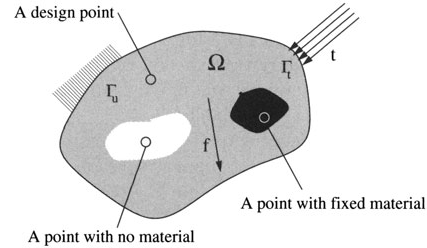
\includegraphics[width=0.6\textwidth]{Pictures/TopOp/design_domain.png}
\caption{The reference domain $\Omega$ for the minimum compliance problem. The problem is formulated such that for a set of external loads $t$ on boundaries $\lambda_t$, body forces $f$ and a set of fixed support points $\lambda_u$, the material distribution within $\Omega$ is such that the stiffness with regards to these loads and forces is maximal and the energy stored by the application of those forces is minimal. The problem also allows defining areas which either cannot or must be filled with material. Figure taken from \cite{bendsoe2003topology}.}
\label{fig:topOpRefDomain}
\end{figure}
In order to constrain the resulting structure as little as possible, the formulation of the topology optimization problem is generally given as follows: for a given set of external fixture points, external loads and/or body forces, the distribution of material within the reference domain should be found such that the structure has maximum stiffness. This is obtained when the structure has the minimum energy stored by external work for the applied forces. The problem is also usually formed to allow for regions in the domain to be specified as filled or empty of material (see \autoref{fig:topOpRefDomain}). The formulation allows the problem to be cast as finding a displacement field $u$ and a stiffness tensor field $E$ that is in equilibrium with the applied loads, and that minimizes the external work done by the forces. 

To turn this into a more tractable mathematical problem, a few physical assumptions are also typically made: that the material is isotropic, and that it is linearly elastic. From the assumptions of isotropy and linear elasticity of the material, the stiffness field becomes a constant of the material, defined where there is material in the domain. The problem is also easy to cast into a weak form. First of all, we compute the integrated internal virtual work and external work. The former is the work of deforming the elastic material from equilibrium by an admissible displacement. External work is done by the loads and forces to bring out this displacement. Having computed these, we set them equal to one another in order to conserve energy. As a result we obtain an equation that relates the equilibrium displacement, stiffness tensor, and the forces and loads. We then cast this into the weak form, which can be solved using Finite Element Methods (FEM). These can also incorporate the calculation of the external work done.

\subsubsection{SIMP: Solid Isotropic Material with Penalization}
However, in trying to minimise this external work done by looking at different material distributions, the usual problem of finding an optimum arises: where to look? After discretising the domain with FEM, the possibilities of where to put material at least aren't infinite - but they still grow exponentially with the number of elements, so trying out one-by-one is not going to prove efficient. One popular way of recasting the problem to allow for easier solving is the SIMP model, where instead of either being present or not at a point, the material presence can take a continous set of values between one and zero -- as some kind of density, fixing the total final volume by integrating this density over the domain, instead of constraining the allowed occupied space. In order to still obtain topologies where material is predominantly in certain areas -- of densities one, with the rest being empty at densities close to zero -- a "penalty" is applied to the intermediate values. This is effected by raising the density to a power $> 1$ in the elastic energy calculation, but not in the volume calculation, such that an intermediate density value provided less elastic support, but still "costs" as much volume, and will thus be suboptimal. 

In typical implementations, a heuristic iterative scheme is then used for finding a solution. The optimal solution is assumed to have all present parts stressed (as they would otherwise be unnecessary, not providing any support). Thus, at places where the elastic energy is high, material is added if possible, and where it is low, material is likewise removed, with the values "high" and "low" being determined dynamically to keep the total volume constraint. 

This whole scheme is one of the simpler topology optimisation schemes to implement, and has been done so in several pieces of open-source software, including a known 99-line Matlab code by Sigmund \cite{sigmund200199}and ToPy described in \autoref{sec:ToPy} below. For an extended explanation and discussion, as well as further alternative methods for topology optimisation, the interested reader is referred to \cite{bendsoe2003topology}.


%Maybe a little theory here about how topology optimization actually works

\subsection{ToPy library}\label{sec:ToPy}
ToPy \cite{ToPy} is a python library/program, written by William Hunter and documented in \cite{Hunter2009}, implementing the SIMP model and method described above. It is based on the 99-line Matlab code by Sigmund's for minimum compliance \cite{sigmund200199}. The program can optimize the three above named problem types, minimum compliance, heat conduction and mechanism synthesis-- in 2D as well as 3D. It uses available open source python software, as for example Pysparse and Numpy, leading to improved speed, porta- and scalability. The whole program is steered by an input file which-- with the help of the documentation-- is straightforward to use and easy to adapt. 

\subsection{Implementation}
In terms of our implementation, we use ToPy as a blackbox topology optimizer. This means, we launch the program with an input file based on our scenario, let ToPy run and proceed by working with the output of ToPy. The intention is to touch the solver itself as less as possible to be able to just plug in different solvers later on. Implementation-wise that means, that we wrote a program which takes as input a voxelized CAD design in, for example, stl-format and outputs a tpd-file which can be used by ToPy. Results of the process can be seen in figure \ref{fig: topyStar}. Here, a star was given as input from a stl-file. We fixed the voxels in the corners of the structure, while we set a load in the middle, pointing into the structure. As can be seen, the optimization process "cuts" away unnecessary material in-between the corners and even in the middle of the material and returns stiff structure for a minimal amount of material. 
\begin{figure}
\centering
\begin{subfigure}{
  
\includegraphics[width=.2\linewidth]{Pictures/TopOp/Star_Optimized0_Trans.png}}
\end{subfigure}%
\begin{subfigure}{
  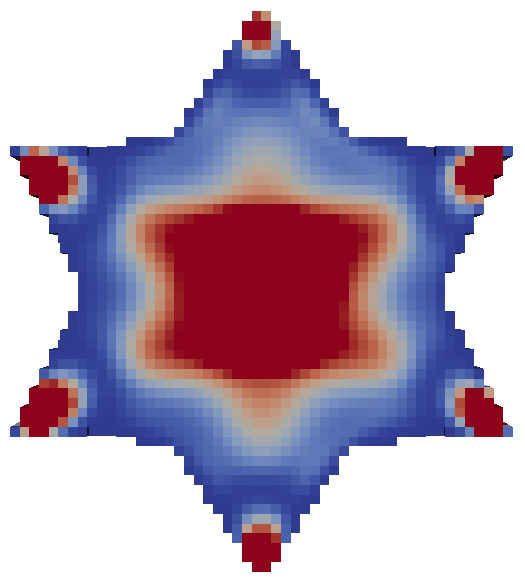
\includegraphics[width=.2\linewidth]{Pictures/TopOp/Star_Optimized2_Trans.png}}
\end{subfigure}
\begin{subfigure}{
  
\includegraphics[width=.2\linewidth]{Pictures/TopOp/Star_Optimized4_Trans.png}}
\end{subfigure}
\begin{subfigure}{
  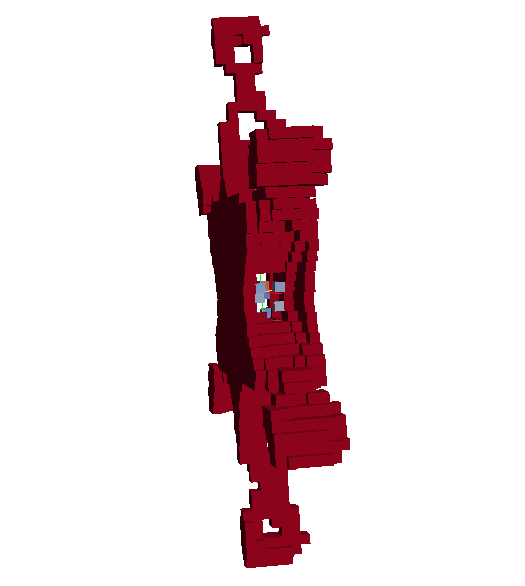
\includegraphics[width=.2\linewidth]{Pictures/TopOp/Star_Optimized5_Trans.png}}
\end{subfigure}
\caption{Topology Optimization with minimum compliance of a star structure, given by an stl-file. The fixtures were applied in the corners of the star, while a load was set in the middle.}
\label{fig: topyStar}
\end{figure}
